\section{Resultados}
En la figura \ref{fig: phase plot x} 
se presenta el diagrama fase del sistema para
posición y velocidad con respecto al eje $x$.




\begin{figure}[h]
 \centering
 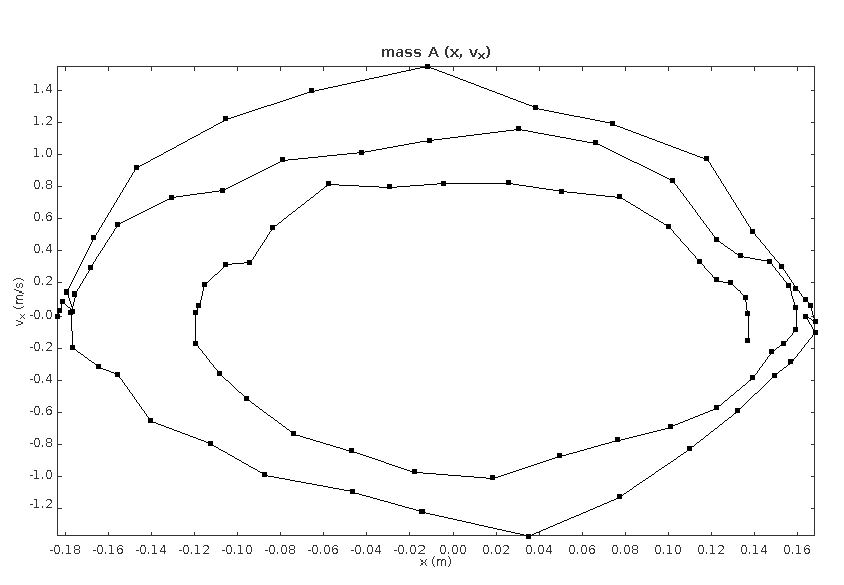
\includegraphics[scale=0.3]{./img/tracker_poc_phasediagram_x_vx.png}
 % tracker_poc_phasediagram_x_vx.png: 844x585 px, 72dpi, 29.78x20.64 cm, bb=0 0 844 585
 \caption{Diagrama de fase del modelo físico para $x$ y $\dot{x}$}
 \label{fig: tracker phase diagram x vx}
\end{figure}

\begin{figure}[h]
 \centering
 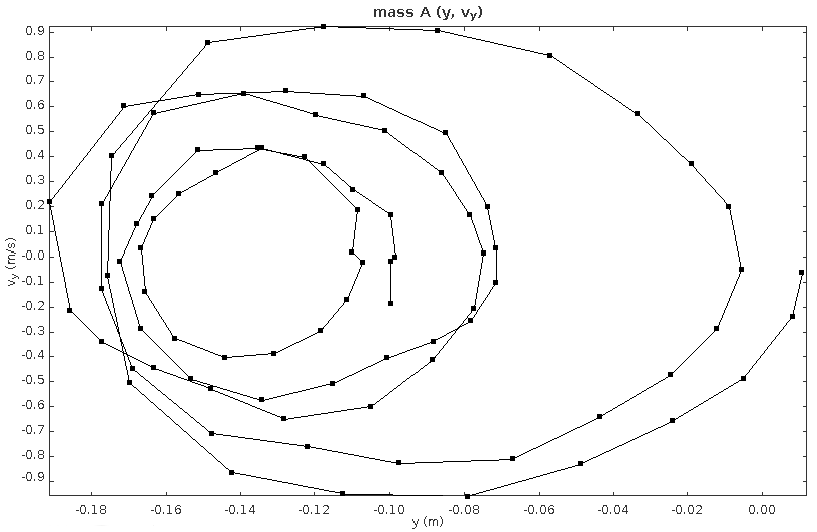
\includegraphics[scale=0.3]{./img/tracker_poc_phasediagram_y_vy.png}
 % tracker_poc_phasediagram_x_vx.png: 844x585 px, 72dpi, 29.78x20.64 cm, bb=0 0 844 585
 \caption{Diagrama de fase del modelo físico para $y$ y $\dot{y}$}
 \label{fig: tracker phase diagram y vy}
\end{figure}


\begin{figure}[h]
 \centering
 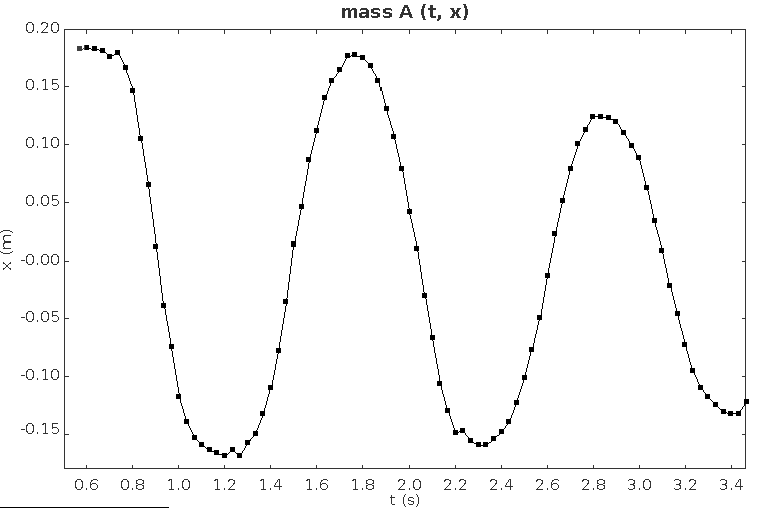
\includegraphics[scale=0.3]{./img/tracker_poc_timeplot_x.png}
 % tracker_poc_phasediagram_x_vx.png: 844x585 px, 72dpi, 29.78x20.64 cm, bb=0 0 844 585
 \caption{Diagrama de tiempo del modelo físico para $x$.}
 \label{fig: tracker time diagram x}
\end{figure}
